\documentclass{standalone}
\usepackage{tikz}
\begin{document}
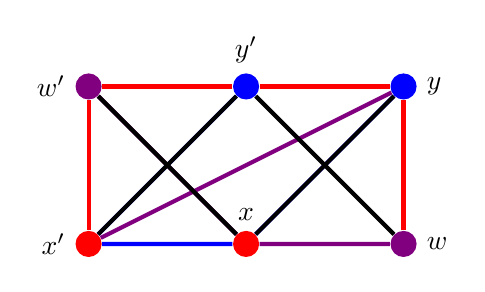
\begin{tikzpicture}
    % Define the nodes
    \node[label=180:{$w'$}, circle, fill=violet] (w') at (0, 2) {};
    \node[label=180:{$x'$}, circle, fill=red] (x') at (0, 0) {};
    \node[label=90:{$y'$}, circle, fill=blue] (y') at (2, 2) {};
    \node[label=90:{$x$}, circle, fill=red] (x) at (2, 0) {};
    \node[label=0:{$y$}, circle, fill=blue] (y) at (4, 2) {};
    \node[label=0:{$w$}, circle, fill=violet] (w) at (4, 0) {};

    % Draw the edges
    \draw[red, line width=1.5pt] (w') -- (x') -- (x) -- (w) -- (y) -- (y') -- (w');
    \draw[blue, line width=1.5pt] (y') -- (x') -- (x) -- (y);
    \draw[violet, line width=1.5pt] (w') -- (x) -- (w);
    \draw[violet, line width=1.5pt] (x') -- (y);
    \draw[line width=1.5pt] (w') -- (x) -- (y) -- cycle; % This adds the black edges
    \draw[line width=1.5pt] (x') -- (y') -- (w) -- cycle; % This adds the black edges

    % Add additional textual annotations if necessary
    \node[violet] at (0, 2.3) {}; % You can add labels or descriptions similarly if needed, but here it's just for reference
\end{tikzpicture}
\end{document}